\documentclass[x11names, crop, tikz]{standalone}
\usepackage{tikz}
\usepackage{xcolor}

\begin{document}\thispagestyle{empty}

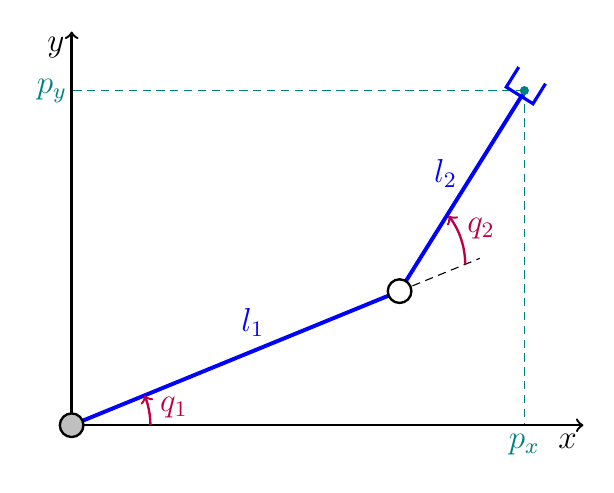
\begin{tikzpicture}


\draw[teal, densely dashed] (5.75, 4.25) -- (0, 4.25);
\draw[teal, densely dashed] (5.75, 4.25) -- (5.75,0);
\draw(-0.25,4.25) node[align=left] {\large \textcolor{teal}{$p_y$}};
\draw(5.75,-0.25) node[align=left] {\large \textcolor{teal}{$p_x$}};


\draw[densely dashed] (4.165,1.703) -- (5.183,2.119);

\draw[line width=0.3mm, black, arrows=->] (0,0) -- (0,5);
\draw[line width=0.3mm, black, arrows=->] (0,0) -- (6.5,0);
\draw(6.3,-0.2) node[align=left] {\large $x$};
\draw(-0.2,4.8) node[align=left] {\large $y$};

\draw[line width=0.5mm, blue] (0,0) -- (4.165,1.703);
\draw[line width=0.5mm, blue] (4.165,1.703) -- (5.77, 4.27);

% origin
\filldraw[line width=0.3mm, draw=black, fill=gray!50] (0,0) circle (1.5mm);

% first solution
\filldraw[line width=0.3mm, draw=black, fill=white] (4.165,1.703) circle (1.5mm);

% second solution
%\filldraw[line width=0.3mm, draw=black, fill=white] (2.85, 3.483) circle (1.5mm);

% actuator
\filldraw[draw=teal, fill=teal] (5.75,4.25) circle (0.5mm);

%\filldraw[line width=0.2mm] (5.75, 4.25) circle (1.5mm);
\begin{scope}[xshift=51.5mm, yshift=37mm]
\draw[rotate=58.12, line width=0.4mm, draw=blue] (1,0) -- (0.7,0) -- (0.7,-0.4) -- (1,-0.4);
\end{scope}
%\begin{scope}[xshift=52mm, yshift=38mm]
%\draw[rotate=58.12, line width=0.4mm, draw=blue] (1,0) -- (0.7,0) -- (0.7,-0.4) -- (1,-0.4);
%\end{scope}

\draw[draw=purple, line width=0.3mm, ->] (1,0) arc(0:22.231:1cm);
\draw(1.3,0.225) node {\large\textcolor{purple}{$q_1$}};

\draw[draw=purple, line width=0.3mm, ->] (4.998,2.044) arc(0:38:1cm);
\draw(5.2,2.5) node {\large\textcolor{purple}{$q_2$}};


\draw(2.3,1.3) node {\large\textcolor{blue}{$l_1$}};
\draw(4.75,3.2) node {\large\textcolor{blue}{$l_2$}};


\end{tikzpicture}

\end{document}
